\documentclass[a4paper,12pt]{article}
\usepackage{graphicx}
\usepackage{epstopdf}
\usepackage{gensymb}
\usepackage{longtable}
%% Definitioner för LIPS-dokument

\usepackage[swedish]{babel}
\usepackage[utf8]{inputenc}
\usepackage[T1]{fontenc}
\usepackage{times}
\usepackage{ifthen}

\usepackage[margin=25mm]{geometry}

\usepackage{fancyhdr}
\pagestyle{fancy}
\lhead{}
\chead{\textbf{\LIPSprojekttitel}}
\rhead{\textbf{\textsl{LiTH}}\\\textbf{\LIPSdatum}}
\lfoot{\textbf{\LIPSkursnamn}\\\textbf{\LIPSdokumentansvarig}}
\cfoot{\textbf{\LIPSprojektgrupp}\\\textbf{\LIPSgruppepost}}
\rfoot{\textbf{\textsc{Lip}s}\\\textbf{Sida~\thepage}}

\setlength{\parindent}{0pt}
\setlength{\parskip}{1ex plus 0.5ex minus 0.2ex}


\newcommand{\twodigit}[1]{\ifthenelse{#1<10}{0}{}{#1}}
\newcommand{\dagensdatum}{\number\year-\twodigit{\number\month}-\twodigit{\number\day}}

%% ------------------------------------------
% NYBILD
% Skapar centrerad bild med caption
%   
% #1: Filens url relativt '/bilder/'
% #2:  Caption
% #3: Label
% #4: Skalning
%% ------------------------------------------
\newcommand{\nyBild}[4] 
{\begin{figure}[H]
  \centering
 \includegraphics[angle=0,scale=#4]{bilder/#1}
  \caption{#2}
  \label{fig:#3}
\end{figure}}



%%  Redefinitions of commands containing @
\makeatletter
\makeatother

\newcommand{\LIPStitelsida}{%
{\ }\vspace{45mm}
\begin{center}
  \textbf{\Huge \LIPSdokumenttyp}
\end{center}
\begin{center}
  {\Large Redaktör: \LIPSredaktor}
\end{center}
\begin{center}
  {\Large \textbf{Version \LIPSversion}}
\end{center}
\vfill
\begin{center}
  {\large Status}\\[1.5ex]
  \begin{tabular}{|*{3}{p{40mm}|}}
    \hline
    Granskad & \LIPSgranskare & \LIPSgranskatdatum \\
    \hline
    Godkänd & \LIPSgodkannare & \LIPSgodkantdatum \\
    \hline
  \end{tabular}
\end{center}
\newpage
}


\newenvironment{LIPSprojektidentitet}{%
{\ }\vspace{45mm}
\begin{center}
  {\Large PROJEKTIDENTITET}\\[0.5ex]
  {\small
  \LIPSartaltermin, \LIPSprojektgrupp\\
  Linköpings Tekniska Högskola, ISY
  }
\end{center}
\begin{center}
  {\small Gruppdeltagare}\\
%  \begin{tabular}{|p{30mm}|p{40mm}|p{35mm}|p{45mm}|}
  \begin{tabular}{|l|p{45mm}|p{25mm}|l|}
    \hline
    \textbf{Namn} & \textbf{Ansvar} & \textbf{Telefon} & \textbf{E-post} \\
    \hline
}%
{%
    \hline
  \end{tabular}
\end{center}
\begin{center}
  {\small
    \textbf{E-postlista för hela gruppen}: \LIPSgruppepost\\
    \textbf{Hemsida}: \LIPSgrupphemsida\\[1ex]
    \textbf{Kund}: \LIPSkund\\
    \textbf{Kontaktperson hos kund}: \LIPSkundkontakt\\
    \textbf{Kursansvarig}: \LIPSkursansvarig\\
    \textbf{Handledare}: \LIPShandledare\\
  }
\end{center}
\newpage
}
\newcommand{\LIPSgruppmedlem}[4]{\hline {#1} & {#2} & {#3} & {#4} \\}



\newenvironment{LIPSdokumenthistorik}{%
\begin{center}
  Dokumenthistorik\\[1ex]
  \begin{small}
    \begin{tabular}{|l|l|p{60mm}|l|l|}
      \hline
      \textbf{Version} & \textbf{Datum} & \textbf{Utförda förändringar} & \textbf{Utförda av} & \textbf{Granskad} \\
      }%
    {%
      \hline
    \end{tabular}
  \end{small}
\end{center}
}
\newcommand{\LIPSversionsinfo}[5]{\hline {#1} & {#2} & {#3} & {#4} & {#5} \\}

\newcounter{LIPSkravnummer}
\newcounter{LIPSunderkravnummer}[LIPSkravnummer]
\newenvironment{LIPSkravlista}{%
  \begin{tabular}{|p{25mm}|p{25mm}|p{85mm}|p{5mm}|}
    }%
  {%
    \hline
  \end{tabular}
}
\newcommand{\LIPSkrav}[3]{\hline\stepcounter{LIPSkravnummer}\textbf{Krav nr \arabic{LIPSkravnummer}} & \textbf{{#1}} & {#2} & \textbf{{#3}} \\}
\newcommand{\LIPSunderkrav}[3]{\hline\stepcounter{LIPSunderkravnummer}\textbf{Krav nr \arabic{LIPSkravnummer}\Alph{LIPSunderkravnummer}} & \textbf{{#1}} & {#2} & \textbf{{#3}} \\}





%%% Local Variables: 
%%% mode: latex
%%% TeX-master: "kravspec_mall"
%%% End: 



\newcommand{\LIPSartaltermin}{2012/VT}
\newcommand{\LIPSkursnamn}{TSEA27}

\newcommand{\LIPSprojekttitel}{Komborobot}

\newcommand{\LIPSprojektgrupp}{Grupp 17}
\newcommand{\LIPSgruppepost}{komborobot@googlegroups.com}
\newcommand{\LIPSgrupphemsida}{finns ej}
\newcommand{\LIPSdokumentansvarig}{Mattias Jansson}

\newcommand{\LIPSkund}{ISY, Linköpings universitet, 581\,83 Linköping}
\newcommand{\LIPSkundkontakt}{Tomas Svensson, 013-281368, tomass@isy.liu.se}
\newcommand{\LIPSkursansvarig}{Tomas Svensson, 013-281368, tomass@isy.liu.se}
\newcommand{\LIPShandledare}{Olov Andersson, 013-282658, olov@isy.liu.se}


\newcommand{\LIPSdokumenttyp}{Projektplan}
\newcommand{\LIPSredaktor}{Simon Larsson}
\newcommand{\LIPSversion}{1.1}
\newcommand{\LIPSdatum}{\dagensdatum}

\newcommand{\LIPSgranskare}{Markus Falck}
\newcommand{\LIPSgranskatdatum}{\dagensdatum}
\newcommand{\LIPSgodkannare}{Tomas Svensson}
\newcommand{\LIPSgodkantdatum}{2012-02-23}

\begin{document}

\LIPStitelsida

%% Argument till \LIPSgruppmedlem: namn, roll i gruppen, telefonnummer, epost
\begin{LIPSprojektidentitet}
  \LIPSgruppmedlem{Simon Larsson}{Projektledare (PL)}{070-7311646}{simla804@student.liu.se}
  \LIPSgruppmedlem{\LIPSdokumentansvarig}{Dokumentansvarig (DOK)}{073-6837074}{matja307@student.liu.se}
  \LIPSgruppmedlem{Gustav Svensk}{Reglersystem (REG)}{073-6208776}{gussv666@student.liu.se}
  \LIPSgruppmedlem{Johan Jönsson}{Mjukvara (KA)}{073-8305758}{johjo939@student.liu.se}
  \LIPSgruppmedlem{Tobias Andersson}{Hårdvara (HV)}{073-7201098}{toban963@student.liu.se}
  \LIPSgruppmedlem{Markus Falck}{Leveransansvarig (LV)}{076-3457552}{marlo265@student.liu.se}
  \LIPSgruppmedlem{Simon Wallin}{Testansvarig (GM)}{076-2300665}{simwa252@student.liu.se}
\end{LIPSprojektidentitet}

\tableofcontents{}
\newpage

%% Argument till \LIPSversionsinfo: versionsnummer, datum, ändringar, utfört av, granskat av
\addcontentsline{toc}{section}{Dokumenthistorik}
\begin{LIPSdokumenthistorik}
  \LIPSversionsinfo{0.1}{2012-02-15}{Första utkast.}{matja307}{marlo265}
  \LIPSversionsinfo{0.2}{2012-02-22}{Komplettering av utkast.}{simla804}{}
  \LIPSversionsinfo{1.0}{2012-02-23}{Första versionen}{simla804}{matja307}
  \LIPSversionsinfo{1.1}{2012-03-19}{Aktivitetslista uppdaterad}{simwa252}{simla804}
\end{LIPSdokumenthistorik}
\newpage


\section{Beställare} %%SL
Projektets beställare är Tomas Svensson vid institutionen för systemteknik vid Linköpings universitet.

\section{Översiktlig beskrivning av projektet} %%Markus

\subsection{Syfte och mål}

Syftet med detta projektarbete är att konstruera en robot som på ett tillfredsställande vis uppfyller de krav som
som finns specificerade i projektets kravspecifikation. Projektgruppen förbinder sig att senast under vecka 20, år 2012, ha en
färdig produkt att leverera. Projektgruppen syftar till att utföra projektet på ett metodiskt och professionellt vis.

I samband med leveransen ska roboten klara av att under tävling helt autonomt navigera en bana som är uppbyggd enligt bestämmelserna i  bifogad banspecifikation se~\ref{app:bana}. Tävlingen avgörs på tid, den robot som tar sig runt banan på kortast tid vinner. 

Projektet är lejonparten i kursen TSEA27  som är en obligatorisk kurs på civilingenjörsutbildningen i teknisk fysik \& elektroteknik vid Linköpings universitet. Projektgruppens mål är också att ta till sig de kunskaper denna kurs syftar till att förmedla angående till exempel projektorganisatoriska färdigheter. 
 
\subsection{Leveranser}
Nedan följer en lista över alla dokument som kommer att skrivas under projektets gång. Med ''Ansvarig'' åsyftas den medlem i projektgruppen som är ytterst ansvarig för att dokumentet skrivs och är av god standard. Rubriken ''Godkänns av'' syftar på den person utanför projektgruppen som beslutar huruvida dokumentet är godkänt eller ej. Under ''Syfte'' så beskrivs kort vad dokumentet innehåller. Datumet är deadline för de olika dokumenten. 

Alla dokument kommer att distribueras till projektgruppen, samt till den person som nämns under ''Godkänns av''.


\begin{tabular}{|p{43mm}|p{15mm}|p{70mm}|p{23mm}|}
\LIPSleverans{\textbf{Leverans}}{\textbf{Ansvarig / Godkänns av}}{\textbf{Syfte}}{\textbf{Färdig-datum}}
\LIPSleverans{Första version av Projektplan, tidplan och systemskiss}{Simon L / Tomas}{Beskriver hur projektet ska utföras och ger en handvisning till hur roboten ska fungera}{15/2-2012}
\LIPSleverans{Slutgiltig version av Projektplan, tidplan och systemskiss}{Simon L / Tomas}{Beskriver hur projektet ska utföras och ger en handvisning till hur konstruktionen av roboten ska ske}{23/2-2012}
\LIPSleverans{Första version av designspecifikation}{Johan / Olov}{Visar mer detaljerat hur konstruktionen av roboten ska ske}{13/3-2012}
\LIPSleverans{Slutgiltig version av designspecifikation}{Simon L / Olov}{Visar mer detaljerat hur konstruktionen av roboten ska ske}{16/3-2012}
\LIPSleverans{Tidrapporter och uppdaterad tidplan}{Simon L / Tomas}{Visar hur tidfördelningen mellan de olika aktiviteterna har gått under den senaste tidsperioden, samt hur projektgruppen tänkt lägga upp sitt framtida arbete}{12/3, 19/3, 26/3, 2/4, 16/4, 23/4, 30/4, 7/5, 14/5, 21/5}
\LIPSleverans{Statusrapport för projektet}{Simon L / Tomas}{Ger en bild av projektgruppens nuvarande status i förhållande till tidigare planering}{Vid begäran}
\LIPSleverans{Teknisk dokumentation och användaranvisning}{Gustav / Tomas}{Ger en detaljerad bild över hur systemet fungerar, information om användargränssnit och beskrivning hur roboten används}{Tre arbetsdagar innan redovisningen vecka 20}
\LIPSleverans{Muntlig presetation och demonstration}{Simon L / Tomas}{Slutleveransen som består av en 15-20 minuter lång presentation av robotens specifikationer och funktioner}{Vecka 20}
\LIPSleverans{Leverans av robot}{Markus / Tomas}{En robot som uppfyller ställda krav levereras till beställaren}{vecka 20, 2012}
\LIPSleverans{Efterstudie}{Simon L / (delges senare)}{Projektgruppen sammanställer här sina erfarenheter från projektarbetet och lämnar synpunkter på hur projektkursen skulle kunna förändras}{1/6-2012}
\hline
\end{tabular}




\subsection{Begränsningar}
Projektarbetet begränsas till att uppfylla de krav som finns specificerade i projektets kravspecifikation. I denna finns tre olika prioriteringsnivåer för vad roboten ska kunna uppnå vid slutleverans. Projektet begränsas till att endast i mån av tid hantera de krav med prioritering 2 och 3.
Den kanske viktigaste begränsningen av projektgruppens arbete är att efter det att projektplanen blivit godkänd får endast 140 timmar per projektmedlem användas till projektet.


Vilka komponenter som ska användas vid konstruktionen av roboten är begränsat av utbudet i ISY's komponentbibliotek. Märk dock att denna begränsning inte är strikt, vid behov av ytterligare komponenter kan eventuellt beställning från extern part göras efter en diskussion med beställare och handledare. 


\section{Fasplan}		

\subsection{Under projektet}
Under projektets gång ligger huvudfokus på att konstruera komboroboten samt att framställa den dokumentation som beställaren kräver. Dessutom läggs en del av tiden på laborationer och utbildning av gruppmedlemar.
\subsection{Efter projektet}
När roboten är klar för leverans skall den delta i en tävling där den skall visa att den uppfyller kraven. Efter tävlingen beslutar beställaren om projektet godkänns eller ej. En efterstudie ska genomföras av samtliga projektmedlemar, och rapport på denna ska lämnas in till beställaren. 

\section{Organisationsplan för hela projektet}	%%SL
\begin{figure}[h]
        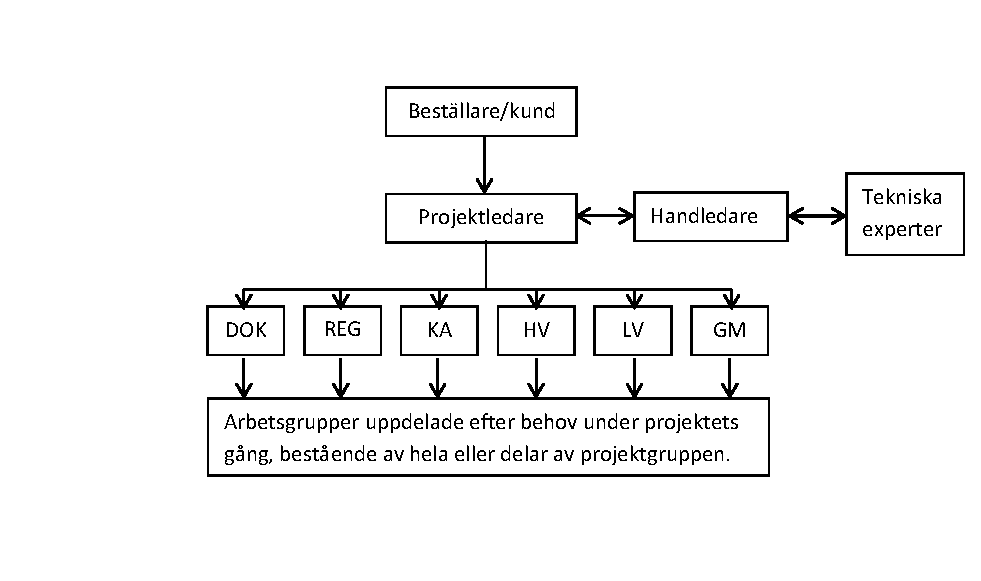
\includegraphics{organisation-figur.pdf}
	\caption{Översikt av ansvarsfördelning}
\end{figure}
Beställarens kontakt med gruppen sker huvudsakligen genom projektledaren. Varje gruppmedlem har ett eget ansvarsområde, och det ligger under projektledarens ansvar att se till att övriga gruppmedlemmar arbetar mot samma mål och att samtliga planerade aktiviteter har minst en huvudansvarig. Projektledaren ansvarar dessutom för att projektgruppen under projektets gång  delas in i mindre arbetsgrupper för att arbetsfördelningen inom gruppen, sett till nedlagda arbetstimmar,  skall bli så jämnt fördelad som möjligt.
Handledaren finns tillgänglig som vägledning för projektgruppen under hela projektets gång. Om gruppen har frågor rörande någon teknisk del av projektet kan handledaren hänvisa till en teknisk expert på området ifråga. Handledaren ska även godkänna vissa beslutspunkter för att projektet ska kunna fortskrida, se "Milstolpar och beslutspunkter".

\subsection{Villkor för samarbete inom projektgruppen}
Se gruppkontrakt (Appendix B)

\subsection{Definition av arbetsinnehåll och ansvar}
Varje medlem i projektgruppen har blivit tilldelat ett ansvarsområde enligt tabellen nedan. Den huvudansvarige för ett område ska se till att aktiviteter inom ansvarsområdet genomförs som planerat och med önskvärt resultat. Alla medlemmar i projektgruppen finns tillgängliga som extra arbetskraft när det finns tid över från det egna huvudområdet.
\\
\\
\begin{tabular}{|p{16mm}|p{31mm}|p{100mm}|}
        	\LIPSmilstolpe{\textbf{Namn}}{\textbf{Ansvarsområde}}{\textbf{Kommentar}}
	\LIPSmilstolpe{Simon L}{Projektledare}{Ansvarar för att projektgruppens sammanlagda arbete går framåt mot uppsatta mål. Uppdaterar tidsplanen och skickar in tidrapport enl. överenskommelse med beställaren}
	\LIPSmilstolpe{Mattias}{Dokumentansvarig}{Ansvarar för alla dokument och möteshandlingar}
	\LIPSmilstolpe{Gustav}{Ansvarig för reglersystem}{Huvudansvarig för robotens styr-och reglersystem}
	\LIPSmilstolpe{Johan}{Mjukvaruansvarig}{Ansvarar för framtagande och optimering av all programmeringskod i projektet.}
	\LIPSmilstolpe{Tobias}{Hårdvaruansvarig}{Ansvarar för konstruktion av nödvändig hårdvara}
	\LIPSmilstolpe{Simon W}{Testansvarig}{Ansvarig för att upprätta en testplan och kontinuerligt genomföra tester enligt denna}
\hline
\end{tabular}

\section{Dokumentplan}	%%MJ
Nedan följer en lista över alla dokument som kommer att skrivas under projektets gång. Med ''Ansvarig'' åsyftas den medlem i projektgruppen som är ytterst ansvarig för att dokumentet skrivs och är av god standard. Rubriken ''Godkänns av'' syftar på den person utanför projektgruppen som beslutar huruvida dokumentet är godkänt eller ej. Under ''Syfte'' så beskrivs kort vad dokumentet innehåller. Färdig-datum syftar till det datum då respektive dokument sk levereras. 

Alla dokument kommer att distribueras till projektgruppen, samt till den person som nämns under ''Godkänns av''.

\begin{tabular}{|p{40mm}|p{20mm}|p{50mm}|p{23mm}|}
\LIPSleverans{\textbf{Dokument}}{\textbf{Ansvarig / Godkänns av}}{\textbf{Syfte}}{\textbf{Färdig-datum}}
\LIPSleverans{Kravspecifikation}{Simon L / Tomas}{Definierar kraven som ställs på projektet}{2/2-2012}
\LIPSleverans{Projektplan, första inlämningnen}{Markus / Tomas}{Beskriver hur projektet ska utföras.}{15/2-2012}
\LIPSleverans{Systemskiss, första inlämningnen}{Markus / Tomas}{Beskriver hur systemet ska byggas upp}{15/2-2012}
\LIPSleverans{Tidplan, första inlämningnen}{Markus / Tomas}{Listar aktiviteternas budgeterade tidsåtgång.}{15/2-2012}
\LIPSleverans{Projektplan, slutgiltig inlämning}{Simon L / Tomas}{Beskriver hur projektet ska utföras.}{23/2-2012}
\LIPSleverans{Systemskiss, slutgiltig inlämning}{Simon L / Tomas}{Beskriver hur systemet ska byggas upp}{23/2-2012}
\LIPSleverans{Tidplan, slutgiltig inlämning}{Simon L / Tomas}{Listar aktiviteternas budgeterade tidsåtgång.}{23/2-2012}
\LIPSleverans{Designspecifikation, första inlämningen}{Johan / Olov}{Visar mer detaljerat hur konstruktionen av roboten ska ske}{13/3-2012}
\LIPSleverans{Designspecifikation, slutlig inlämning}{Simon L / Olov}{Visar mer detaljerat hur konstruktionen av roboten ska ske. Version 1.0 och högre skickas till Tomas}{16/3-2012}
\LIPSleverans{Tidrapporter och uppdaterad tidplan}{Markus / Tomas}{Visar budgeterad och spenderad tid, uppdelad på de olika aktiviteterna}{Måndagar varje vecka, med start 12/3 och slut 21/5-2012 (undantaget 9/4)}
\LIPSleverans{Statusrapport för projektet}{Simon L / Tomas}{Dokumentet ska översiktligt sammanfatta hur projektet fortskrider.}{Vid begäran}
\LIPSleverans{Teknisk dokumentation}{Gustav / Tomas}{Beskriver i detalj systemets uppbyggnad}{Tre arbetsdagar innan redovisningen, vecka 20}
\LIPSleverans{Användaranvisning}{Mattias / Tomas}{Beskriver hur produkten används och dess olika funktioner.}{Tre arbetsdagar innan redovisningen, vecka 20}
\LIPSleverans{Efterstudiedokument}{Simon L / (delges senare)}{Dokumenterar gruppens reflektioner över projektet och hur det har genomförts}{1/6-2012}
\hline
\end{tabular}

%%\section{Utvecklingsmetodik}	%%SW

\section{ Utbildningplan}	%%Markus
\subsection{Egen utbildning}
Vid behov kommer medlemmarna i projektgruppen att kunna utbildas i de olika verktyg som ska användas under projektet. Exempel på sådana verktyg kan vara AVR Studio, C Programmering och alla de mätinstrument som kommer att vara nödvändiga. För att utbilda projektetgruppens medlemmar tillhandahåller beställaren med Tekniska experter som kan ge korta lektioner. Innan någon av de tekniska experterna anlitas kommer projektgruppen dock att tillfråga handledaren om denna kan hålla en kort intern utbildning. 

I den kurs som projektarbetet ingår, TSEA27, finns också andra utbildande moment. Kursen innehåller elva frivilliga föreläsningar som samtliga deltagare i projektgruppen i största möjliga mån ska lyssna på. Fem stycken av dessa föreläsningar handlar om projektets upplägg och projektmodellen LIPS och sex stycken handlar om den teknik som kan användas för att konstruera roboten.

Samtliga av projektgruppens deltagare kommer också att deltaga på tre stycken laborationer som är obligatoriska moment i projektkursen. Dessa laborationer är utbildande moment och syftar till att förbereda projektgruppen för uppgiften.


\subsection{Kundens utbildning}
Den information som är nödvändig för att använda roboten kommer att finnas i den användaranvisning som ska levereras tillsammans med den tekniska specifikationen senast tre dagar innan presentationen vecka 20. Annan utbildning av kunden anses vara inte nödvändig.


\section{Mötesplan}
Möten för hela gruppen sker om inget annat bestämts på måndagar under schemalagd tid för TSEA27/projektarbete. Under dessa möten skall främst tidsplanen diskuteras och uppdateras. Om inget annat sägs är mötets längd en timme.
Projektledaren skall informera övriga gruppmedlemmar om tid och plats för möte samt kalla till extra gruppmöten för när detta behövs, t.ex. inför en dellerverans eller om projektplaneringen eller krav i kravspecifikationen behöver tas upp till diskussion. Dessutom kan ansvarig för ett delområde inom projektet kalla till möte för hela eller delar av projektgruppen för att planera arbetet. Möten hålls så korta som möjligt för att undvika onödig tidsförbrukning.


\section{Resursplan}	%%SW
Detta avsnitt beskriver de resurser som projektgruppen har att tillgå samt de som är nödvändiga för att projektet ska kunna genomföras. De resurser som kommer att behandlas i avsnittet är personal, material så som kretsar, datorer osv, vilka lokaler som kommer att finnas tillgängliga, hur många timmar som gruppmedlemmarna kan lägga samt den hjälp gruppen kommer behöva från experter på området. 
\subsection{Personer}
Gruppen består av sju medlemmar som alla har sina specifika uppgifter. Dessa är Simon Larsson, Simon Wallin, Johan Jönsson, Gustav Svensk, Markus Falck, Mattias Jansson, Tobias Andersson. Dessa personer kommer att se till att projektet tar sig framåt, att tiden blir allokerad på lämpligt sätt och det är deras ansvar att deadline för beslutspunkterna följs. Utöver detta är även projekthandledaren, Olov, del av projektet. Handledaren ska inte göra något direkt arbete i projektet, utan däremot hjälpa till med att styra projektet åt rätt riktning och ha en administrativ översikt. Han kan också hjälpa till om projektmedlemmarna stöter på något problem. Kontinuerliga möten med handledaren kommer att ske under projektets gång.
\subsection{Materiel}
Allt det material som kommer behövas till projektet kommer att tillhandahållas av ISY. Till detta kommer även all användardata så som manualer och datablad till chip finnas tillgängliga. ISY kommer även att stå för övrig materiel som behövs för att slutför projektet så som hjulbas, sensorer osv.
\subsection{Lokaler}
Den lokal vi huvudsakligen kommer att använda är MUXEN där vi kommer att ha tillgång till en plats för att bygga och programmera vår robot. Dessutom har gruppen tillgång till ett skåp i MUXEN, samt 3 nycklar till skåpet. Vi kommer att ha tillgång till MUXEN 24 timmar om dygnet. 
\subsection{Ekonomi}
Vår ekonomi vi har är i utförandet av timmar vi kan förbruka på projektet. Var person i projektgruppen kommer att ha totalt 140 timmar att spendera på olika aktiviteter vilket sammanlagt ger oss 980 timmar till projektet.


\section{ Milstolpar och beslutspunkter} %%SL
Milstolpar för projektet bestäms inom gruppen, och sätts för att kunna kontrollera att tidsplanen följs som planerat. Varje milstolpe innefattar ett eller flera krav som ska vara uppfyllda och testade vid det datum som specificerats nedan. Beslutspunkter är krav uppsatta från beställaren. Vid varje beslutspunkt har beställaren rätt att besluta om projektet skall fortsätta eller ej.
\subsection{Milstolpar}

\begin{tabular}{|p{7mm}|p{117mm}|p{23mm}|}
        	\LIPSmilstolpe{\textbf{Nr}}{\textbf{Beskrivning}}{\textbf{Datum}}
	\LIPSmilstolpe{1}{Designspecifikationen accepterad av handledaren}{2012-03-16}
	\LIPSmilstolpe{2}{Bussen fungerar som den ska}{2012-03-23}
	\LIPSmilstolpe{3}{Data och mätvärden skickas via komunikationsenheten}{2012-04-30}
	\LIPSmilstolpe{4}{Roboten kan upptäcka korsningar}{2012-04-19}
	\LIPSmilstolpe{5}{Korrekt sensorinfo visas på PCn}{2012-04-20}
	\LIPSmilstolpe{6}{Motorn regleras autonomt utifrån sensorvärdena}{2012-04-27}
	\LIPSmilstolpe{7}{Styrkommandon utförs korrekt}{2012-05-04}
\hline
\end{tabular}

\subsection{Beslutspunkter}

\begin{tabular}{|p{7mm}|p{117mm}|p{23mm}|}
        	\LIPSmilstolpe{\textbf{BP}}{\textbf{Beskrivning}}{\textbf{Datum}}
	\LIPSmilstolpe{BP0}{Godkännande av projektdirektiv, beslut att starta förstudie}{2012-01-20}
	\LIPSmilstolpe{BP1}{Godkännande av kravspecifikation, beslut att starta förberedelsefasen}{2012-02-02}
	\LIPSmilstolpe{BP2}{Godkännande av projektplanering, beslut att starta utförandefasen}{2012-02-23}
	\LIPSmilstolpe{BP3}{Godkännande av designspecifikation, beslut att fortsätta utförandefasen}{2012-03-16}
	\LIPSmilstolpe{BP4}{Ej specifierad}{-}
	\LIPSmilstolpe{BP5}{Godkännande av produktens funktionalitet, beslut att leverera}{vecka 19}
	\LIPSmilstolpe{BP6}{Godkännande av leverans, beslut att upplösa projektgruppen}{2012-06-01}
\hline
\end{tabular}
\section{Aktiviteter}

\begin{longtable}{|p{7mm}|p{90mm}|p{23mm}|p{23mm}|}
	\LIPSleverans{\textbf{Nr}}{\textbf{Beskrivning}}{\textbf{Beroende av aktivitet nr}}{\textbf{Beräknad tid (h)}} 
\LIPSaktivitet{Färdigställande av
designspec}{}{44} 
%% SENSOR
	\LIPSaktivitet{Omvandling av analoga signaler till
digitala sådana}{}{12} 
	\LIPSaktivitet{Trösklande av
sensorvärden}{2}{4} 
	\LIPSaktivitet{Hitt skillnaden mellan önskade och
aktuella värden}{3}{4} 
	\LIPSaktivitet{Skicka skilnaden till styrenheten (via
kommunikationsenheten)}{4 \& 10}{14} 
	\LIPSaktivitet{Skicka avstånd i cm till display- och
kommunikationsenheten}{2 \& 10}{12} 
	\LIPSaktivitet{Upptäck
riktningsmarkeringar}{1 \& 2}{20} 
	\LIPSaktivitet{Hantera
riktningsmarkeringar}{6}{20} 
	\LIPSaktivitet{Upptäck korsningar}{2 \&
3}{20} 
%% KOMMUNIKATION
	\LIPSaktivitet{Ordna master som sköter
buss}{}{50} 
	\LIPSaktivitet{Skicka styrinfo till
pc}{15 \& 23 \& 10}{15} 
	\LIPSaktivitet{Skicka sensorinfo till
pc}{5 \& 15 \& 23}{15} 
	\LIPSaktivitet{Ta emot styrkommandon från
pc}{15 \& 23}{15} 
	\LIPSaktivitet{Skicka styrkommando till styrenhet
från kommunikqtionsenhet}{10}{15} 
	\LIPSaktivitet{Fixa blåtand i
kommunikationsenhet}{}{25} 
%% STYRENHET
	\LIPSaktivitet{Ta emot sensorvärden
(Styrenhet)}{10 \& 5}{20} 
	\LIPSaktivitet{Reglera motorer utifrånsensorvärden}{16 \& 19 \& 22}{40} 
	\LIPSaktivitet{Ta emot styrkommandon
(styrenheten)från kommunikationsenheten}{10 \& 24 \& 14}{20} 
	\LIPSaktivitet{Styra motorer (autonomt och manuellt)}{}{40} 
	\LIPSaktivitet{Skicka styrinfo till
kommunikationsenheten från
styrenheten}{10}{20} 
	\LIPSaktivitet{Hantera
specialkommandon}{8 \& 19}{30}
	\LIPSaktivitet{Regulator}{5}{30} 
%% PC 
	\LIPSaktivitet{Fixa blåtand i
pc}{}{25} 
	\LIPSaktivitet{Hämta och skicka styrkommandon från
pc till kommunikationsenheten (Mjukvara)}{15 \& 23}{30} 
	\LIPSaktivitet{Ta emot styrinfo i PC från
kommunikationsenheten}{15 \& 23 \& 20}{20} 
	\LIPSaktivitet{Ta emot sensorinfo}{15 \& 23 \&
6}{20} 
	\LIPSaktivitet{Visa styrinfo på
skärm}{25}{2} 
	\LIPSaktivitet{Visa sensorinfo på
skärm}{26}{2} 
	\LIPSaktivitet{Ordna gränssnitt på
pc}{}{15} 
%% MONTERING OCH TEST
	\LIPSaktivitet{Montering av
avståndssensorer}{}{10} 
	\LIPSaktivitet{Montering av
linjesensorer}{}{10}
	\LIPSaktivitet{Montering}{30 \&
31}{20} 
	\LIPSaktivitet{Utför styrkommandon}{18 \&
21}{30} 
	\LIPSaktivitet{Test av hela systemet}{2-33 \& (35)}{35} 
	\LIPSaktivitet{Kalibrering av
sensorer}{}{20}
	\LIPSaktivitet{Planering och utförande av tester}{}{10}
	\LIPSaktivitet{Test av bussen}{}{10}
	\LIPSaktivitet{Test av kommunikationsenheten}{}{10}
	\LIPSaktivitet{Test av sensorenheten}{}{10}
	\LIPSaktivitet{Test av styrenheten}{}{10}
%% EFTERARBETE OCH DOKUMENTATION
	\LIPSaktivitet{Sammanställa och granska
teknisk dokumentation}{samtliga}{20} 
	\LIPSaktivitet{Sammanställa och granska
Användarmanual}{37}{20} 
	\LIPSaktivitet{Förbereda
redovisning}{38}{15} 
	\LIPSaktivitet{Tidsloggning (ska ske
kontinuerligt)}{}{20} 
	\LIPSaktivitet{Efterstudie}{39}{15}  
	\LIPSaktivitet{Rest / Reservtid}{}{46}
	\LIPSaktivitet{Möten}{}{70} 

\hline
\end{longtable}

\section{Tidplan}
Se  Appendix A.


\section{Kvalitetsplan}	%SL
För att säkerställa att kvalitén på roboten och dokumentationen används två metoder, granskning och tester. Granskning rör all form av dokumentation som ingår i projektet. Dessutom kommer tester att göras kontinuerligt under projektet för att säkerställa att varje aktivitet ger önskat resultat.
\subsection{Granskningar}
Varje ny version av dokumentationen skall granskas av minst en gruppmedlem innan den anses färdig för inlämning. Om inget annat sägs är det dokumentansvarigs (Mattias Jansson) ansvar att dokumentet granskas. Syftet med granskningen är att kontrollera att dokumentet innehåller alla önskade delar och att det inte innehåller några grova språkliga eller utseendemässiga fel.

\subsection{Testplan}
Under projektet kommer tester utföras löpande för att säkerställa att arbetet ger önskat resultat. Gruppmedlemmen som utsetts till testansvarig (Simon Wallin) är ansvarig för att planera och utföra testningen, samt att framställa en testplan som beskriver hur testerna ska genomföras och vilka krav som måste vara uppfyllda för att ett test ska godkännas.



\section{Prioriteringar}
Gruppens målsättning är först och främst att alla krav med högsta prioritet i kravspecifikationen ska uppfyllas. Om tidsbrist eller andra hinder uppstår kontaktas först beställaren för en diskussion om kravets nödvändighet och eventuell revidering av kravspecifikationen. En annan anledning till att ett krav tas upp till diskussion skulle kunna vara att gruppen känner att oproportionerligt mycket arbete läggs ned på ett förhållandevis oviktigt krav, så att detta går ut över övriga aktiviteter och mål med projektet.

\section{Projektavslut} %MARKUS

Under vecka 20 så sker en redovisning då projektgruppen presenterar sin produkt och utför en demonstration. Redovisningen ska vara 15-20 minuter lång och ska innehålla en muntlig presentation av projektets slutprodukt, såväl som en grafisk presentation som visas på en projektor. Även andra av de tillgängliga presentationsverktygen kan komma att användas. Presentationen kommer att utföras av två personer i projektgruppen varav en kommer att vara projektledaren. Övriga deltagare i projektgruppen kommer att finnas på plats för att svara på frågor efter redovisningen.

Senast tre dagar innan presentationen genomförs kommer den tekniska dokumentationen att levereras till beställaren. Denna ska bland annat innehålla detaljerad information om alla olika delsystem i roboten. I den tekniska manualen kommer det också att ingå en användarmanual som beskriver hur roboten ska användas. Den tekniska dokumentationen, projektredovisningen och demonstrationen är de tre komponenter som utgör projektets slutleverans. 

Demonstrationen av roboten kommer att bestå i en tävling där projektgruppens robot ska utmana en konkurrerande projektgrupp som ska bygga en liknande robot. Reglerna för tävlingen har projektgrupperna kommit överens om gemensamt och dessa finns presenterade i Appendix A. En kort sammanfattning av dessa regler är att det vid tävlingstillfället kommer att fastslås vilken typ av bana som robotarna kommer att tävla i, beroende på hur avancerade funktioner projektgrupperna lyckats åstadkomma. De olika banorna finns presenterade i Appendix B. Vinnaren av tävlingen kommer att få sin robot utställd av beställaren och förloraren får montera isär sin robot.

Detta avslutar den aktiva delen av projektet och efter detta påbörjas den så kallade efter-fasen, se mer information under rubrik 3, Fasplan. Under denna fas i projektarbetet ska  projektgruppen utvärdera hur väl arbetet med projektet har gått och vad som skulle varit bättre att göra på annorlunda sätt. Projektets upplägg ska utvärderas och projektgruppen kommer att göra utlåtanden om hur väl kontakten med de olika parter som är involverade i projektarbetet har gått. En annan viktig punkt i denna utvärdering kommer att vara vad projektgruppen har för tips att ge nästa års studenter som ska utföra liknande projektarbeten. Dessa reflektioner, synpunkter och tips ska sammanfattas i en efterstudie som levereras till beställaren senast 1/6-2012. Efter detta datum är projektet avslutat och det enda som återstår är att återlämna den utrustning som projektgruppen tillåtits låna av institutionen för systemteknik.


\newpage
\appendix

\newpage


\addcontentsline{toc}{section}{Referenser}
\begin{thebibliography}{99}
\bibitem{lipskompendiet}\textit{Projektmodellen LIPS - } Svensson, Tomas
\\Studentlitteratur, 2011.
\end{thebibliography}

\end{document} 

%%% Local Variables: 
%%% mode: latex
%%% TeX-master: t
%%% End: 
